\begin{minipage}[t]{0.45\textwidth}
    \exo{Représenter}{TracerSymAxBlanc1}
    
    \begin{figure}[H]
        \centering
        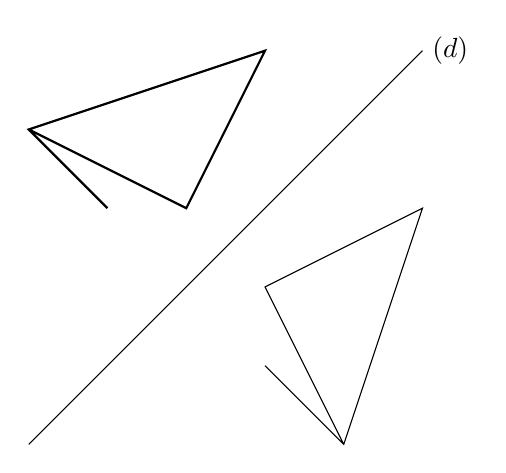
\begin{tikzpicture}
            \def\mypath{(-2,2) -- (-1,1) --(-2,2) -- (1,3)--(0,1)--(-2,2)}
            \draw [thick]\mypath ;
            \draw (-2,-2)--(3,3) node [right]{$(d)$} ;
            \draw [cm={0,1,1,0,(0,0)}] \mypath;%Matrice de transformation inverse X et Y
        \end{tikzpicture}
    \end{figure}
\end{minipage}
\hfill
\begin{minipage}[t]{0.45\textwidth}
    \exo{Représenter}{TracerSymAxBlanc2}
    
    \begin{figure}[H]
        \centering
        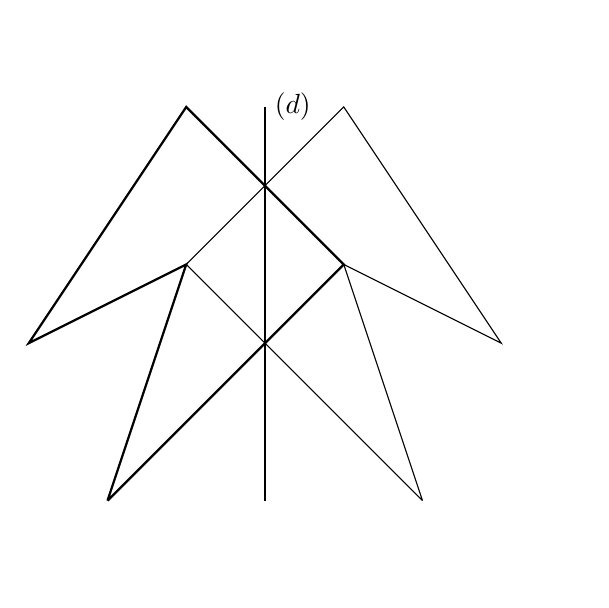
\begin{tikzpicture}
            \def\mypath{(-2,-2) -- (-1,1) --(-3,0) -- (-1,3)--(1,1)--(-2,-2)}
            \draw [white](-3,-3) grid (4,4);
            \draw [thick]\mypath ;
            \draw (0,-2)--(0,3) node [right]{$(d)$} ;
            \draw [cm={-1,0,0,1,(0,0)}] \mypath;%Matrice de transformation inverse X et Y 
        \end{tikzpicture}
    \end{figure}
\end{minipage}

\begin{minipage}[t]{0.45\textwidth}
    \exo{Représenter}{TracerSymAxBlanc3}
    
    \begin{figure}[H]
        \centering
        \begin{tikzpicture}
            \def\mypath{(1,-2) -- (0,-1) --(3,-2) -- (2,-1)--(-1,-1)--(1,-2)}
            \draw [white](-3,-3) grid (4,4);
            \draw [thick]\mypath ;
            \draw (-2,0)--(3,0) node [right]{$(d)$} ;
            \draw [cm={1,0,0,-1,(0,0)}] \mypath;%Matrice de transformation inverse X et Y
        \end{tikzpicture}
    \end{figure}
\end{minipage}
\hfill
\begin{minipage}[t]{0.45\textwidth}
    \exo{Représenter}{TracerSymAxBlanc4}
    
    \begin{figure}[H]
        \centering
        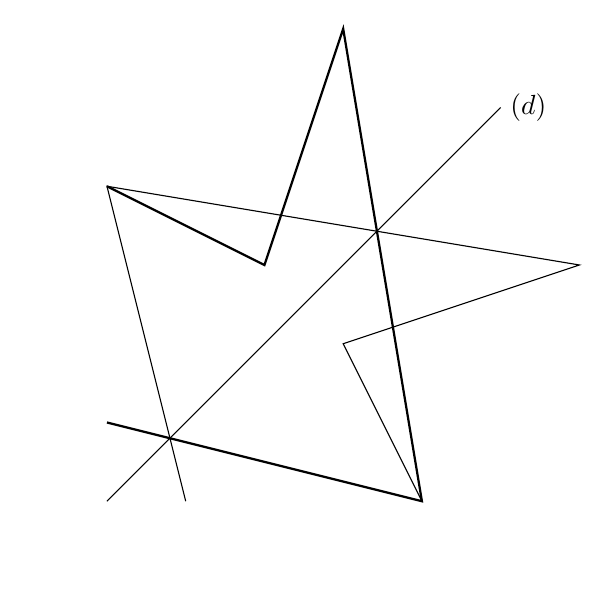
\begin{tikzpicture}
            \def\mypath{(-2,-1) -- (2,-2) --(1,4) -- (0,1)--(-2,2)}
            \draw [white](-3,-3) grid (4,4);
            \draw [thick]\mypath ;
            \draw (-2,-2)--(3,3) node [right]{$(d)$} ;
            \draw [cm={0,1,1,0,(0,0)}] \mypath;%Matrice de transformation inverse X et Y
        \end{tikzpicture}
    \end{figure}
\end{minipage}

\begin{minipage}[t]{0.45\textwidth}
    \exo{Représenter}{TracerSymCentBlanc1}
    
    \begin{figure}[H]
        \centering
        \begin{tikzpicture}
            \tikzset{
                homothety at/.style args={#1 scaled by #2}{shift={($(#1)!#2!(0,0)$)},scale=#2},}
            \def\mypath{(-2,2) -- (-1,1) --(-2,2) -- (1,3)--(0,1)--(-2,2)}
            \draw [white](-3,-3) grid (4,4);
            \draw [thick]\mypath ;
            \fill (0,0) coordinate (c) circle(2pt) node [above] {$O$};
            \begin{scope}[homothety at=c scaled by -1]
                \draw \mypath;
            \end{scope}
        \end{tikzpicture}
    \end{figure}
\end{minipage}
\hfill
\begin{minipage}[t]{0.45\textwidth}
    \exo{Représenter}{TracerSymCentBlanc2}
    
    \begin{figure}[H]
        \centering
        \begin{tikzpicture}
            \tikzset{
                homothety at/.style args={#1 scaled by #2}{shift={($(#1)!#2!(0,0)$)},scale=#2},}
            \def\mypath{(-2,-2) -- (-1,1) --(-3,0) -- (-1,3)--(1,1)--(-2,-2)}
            \draw [white](-3,-3) grid (4,4);
            \draw [thick]\mypath ;
            \fill (1,0) coordinate (c) circle(2pt) node [above] {$O$};
            \begin{scope}[homothety at=c scaled by -1]
                \draw \mypath;
            \end{scope}
        \end{tikzpicture}
    \end{figure}
\end{minipage}

\begin{minipage}[t]{0.45\textwidth}
    \exo{Représenter}{TracerSymCentBlanc3}
    
    \begin{figure}[H]
        \centering
        \begin{tikzpicture}
            \tikzset{
                homothety at/.style args={#1 scaled by #2}{shift={($(#1)!#2!(0,0)$)},scale=#2},}
            \def\mypath{(-2,-2) -- (0,-1) --(3,-2) -- (2,0)--(-1,-1)--(-2,-2)}
            \draw [white](-3,-3) grid (4,4);
            \draw [thick]\mypath ;
            \fill (0,0) coordinate (c) circle(2pt) node [above] {$O$};
            \begin{scope}[homothety at=c scaled by -1]
                \draw \mypath;
            \end{scope}
        \end{tikzpicture}
    \end{figure}
\end{minipage}
\hfill
\begin{minipage}[t]{0.45\textwidth}
    \exo{Représenter}{TracerSymCentBlanc4}
    
    \begin{figure}[H]
        \centering
        \begin{tikzpicture}
            \tikzset{
                homothety at/.style args={#1 scaled by #2}{shift={($(#1)!#2!(0,0)$)},scale=#2},}
            \def\mypath{(-2,-1) -- (2,-2) --(1,4) -- (0,1)--(-2,2)}
            \draw [white](-3,-3) grid (4,4);
            \draw [thick]\mypath ;
            \fill (0,1) coordinate (c) circle(2pt) node [above] {$O$};
            \begin{scope}[homothety at=c scaled by -1]
                \draw \mypath;
            \end{scope}
        \end{tikzpicture}
    \end{figure}
\end{minipage}

\begin{minipage}[t]{0.45\textwidth}
    \exo{Représenter}{TracerTransBlanc1}
    
    \begin{figure}[H]
        \centering
        \begin{tikzpicture}
            \def\mypath{(-2,2) -- (-1,1) --(-2,2) -- (1,3)--(0,1)--(-2,2)}
            \draw [white](-3,-3) grid (4,4);
            \draw [thick]\mypath;
            \draw [shift={(1,-3)}]\mypath ;
            \fill (2,3) coordinate (c) circle(2pt) node [above] {$A$};
            \fill (3,0) coordinate (c) circle(2pt) node [above] {$B$};
        \end{tikzpicture}
    \end{figure}
\end{minipage}
\hfill
\begin{minipage}[t]{0.45\textwidth}
    \exo{Représenter}{TracerTransBlanc2}
    
    \begin{figure}[H]
        \centering
        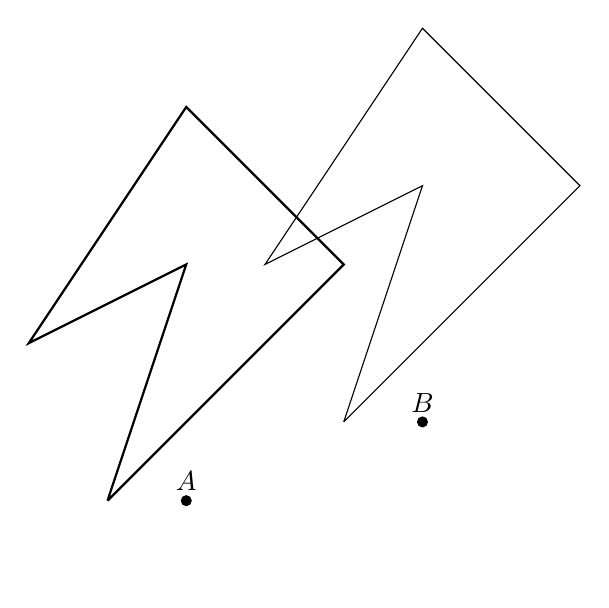
\begin{tikzpicture}
            \def\mypath{(-2,-2) -- (-1,1) --(-3,0) -- (-1,3)--(1,1)--(-2,-2)}
            \draw [white](-3,-3) grid (4,4);
            \draw [thick]\mypath;
            \draw [shift={(3,1)}]\mypath ;
            \fill (-1,-2) coordinate (c) circle(2pt) node [above] {$A$};
            \fill (2,-1) coordinate (c) circle(2pt) node [above] {$B$};
        \end{tikzpicture}
    \end{figure}
\end{minipage}

\begin{minipage}[t]{0.45\textwidth}
    \exo{Représenter}{TracerTransBlanc3}
    
    \begin{figure}[H]
        \centering
        \begin{tikzpicture}
            \def\mypath{(-2,-2) -- (0,-1) --(3,-2) -- (2,0)--(-1,-1)--(-2,-2)}
            \draw [white](-3,-3) grid (4,4);
            \draw [thick]\mypath;
            \draw [shift={(1,3)}]\mypath ;
            \fill (-1,0) coordinate (c) circle(2pt) node [above] {$A$};
            \fill (0,3) coordinate (c) circle(2pt) node [above] {$B$};
        \end{tikzpicture}
    \end{figure}
\end{minipage}
\hfill
\begin{minipage}[t]{0.45\textwidth}
    \exo{Représenter}{TracerTransBlanc4}
    
    \begin{figure}[H]
        \centering
        \begin{tikzpicture}
            \def\mypath{(-2,-1) -- (2,-2) --(1,4) -- (0,1)--(-2,2)}
            \draw [white](-3,-3) grid (4,4);
            \draw [thick]\mypath;
            \draw [shift={(2,1)}]\mypath ;
            \fill (-2,1) coordinate (c) circle(2pt) node [above] {$A$};
            \fill (0,2) coordinate (c) circle(2pt) node [above] {$B$};
        \end{tikzpicture}
    \end{figure}
\end{minipage}


\begin{minipage}[t]{0.45\textwidth}
    \exo{Représenter}{TracerRotaBlanc1}
    
    \begin{figure}[H]
        \centering
        \begin{tikzpicture}
            \def\mypath{(-2,2) -- (-1,1) --(-2,2) -- (1,3)--(0,1)--(-2,2)}
            \draw [white](-3,-3) grid (4,4);
            \draw [thick]\mypath ;
            \fill (0,0) coordinate (c) circle(2pt) node [above] {$0$};
            \draw [rotate=-90] \mypath ;
        \end{tikzpicture}
    \end{figure}
\end{minipage}
\hfill
\begin{minipage}[t]{0.45\textwidth}
    \exo{Représenter}{TracerRotaBlanc2}
    
    \begin{figure}[H]
        \centering
        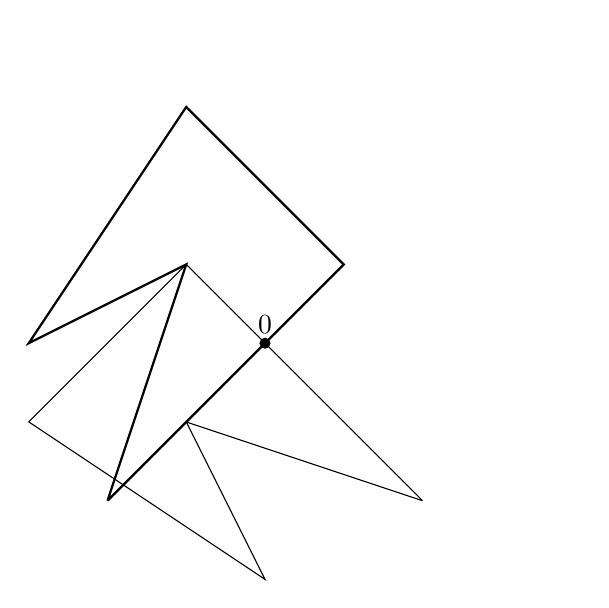
\begin{tikzpicture}
            \def\mypath{(-2,-2) -- (-1,1) --(-3,0) -- (-1,3)--(1,1)--(-2,-2)}
            \draw [white](-3,-3) grid (4,4);
            \draw [thick]\mypath ;
            \fill (0,0) coordinate (c) circle(2pt) node [above] {$0$};
            \draw [rotate=90] \mypath ;
        \end{tikzpicture}
    \end{figure}
\end{minipage}

\begin{minipage}[t]{0.45\textwidth}
    \exo{Représenter}{TracerRotaBlanc3}
    
    \begin{figure}[H]
        \centering
        \begin{tikzpicture}
            \def\mypath{(-2,-2) -- (0,-1) --(3,-2) -- (2,0)--(-1,-1)--(-2,-2)}
            \draw [white](-3,-3) grid (4,4);
            \draw [thick]\mypath ;
            \fill (0,0) coordinate (c) circle(2pt) node [above] {$0$};
            \draw [rotate=-90] \mypath ;
        \end{tikzpicture}
    \end{figure}
\end{minipage}
\hfill
\begin{minipage}[t]{0.45\textwidth}
    \exo{Représenter}{TracerRotaBlanc4}

    
    \begin{figure}[H]
        \centering
        \begin{tikzpicture}
            \def\mypath{(-2,-1) -- (2,-2) --(1,4) -- (0,1)--(-2,2)}
            \draw [white](-3,-3) grid (4,4);
            \draw [thick]\mypath ;
            \fill (0,0) coordinate (c) circle(2pt) node [above] {$0$};
            \draw [rotate=90] \mypath ;
        \end{tikzpicture}
    \end{figure}
\end{minipage}

\begin{minipage}[t]{0.45\textwidth}
    \exo{Représenter}{TracerHomotBlanc1}
    
    \begin{figure}[H]
        \centering
        \begin{tikzpicture}
            \tikzset{
                homothety at/.style args={#1 scaled by #2}{shift={($(#1)!#2!(0,0)$)},scale=#2},}
            \def\mypath{(-2,2) -- (-1,1) --(-2,2) -- (1,3)--(0,1)--(-2,2)}
            \draw [white](-3,-3) grid (5,5);
            \draw [thick]\mypath ;
            \fill (-1,2) coordinate (c) circle(2pt) node [above] {$O$};
            \begin{scope}[homothety at=c scaled by 2]
                \draw \mypath;
            \end{scope}
        \end{tikzpicture}
    \end{figure}
\end{minipage}
\hfill
\begin{minipage}[t]{0.45\textwidth}
    \exo{Représenter}{TracerHomotBlanc2}
    
    
    \begin{figure}[H]
        \centering
        \begin{tikzpicture}
            \tikzset{
                homothety at/.style args={#1 scaled by #2}{shift={($(#1)!#2!(0,0)$)},scale=#2},}
            \def\mypath{(-2,-2) -- (-1,1) --(-3,0) -- (-1,3)--(1,1)--(-2,-2)}
            \draw [white](-3,-3) grid (5,5);
            \draw [thick]\mypath ;
            \fill (0,0) coordinate (c) circle(2pt) node [above] {$O$};
            \begin{scope}[homothety at=c scaled by 1.5]
                \draw \mypath;
            \end{scope}
        \end{tikzpicture}
    \end{figure}
\end{minipage}

\begin{minipage}[t]{0.45\textwidth}
    \exo{Représenter}{TracerHomotBlanc3}
    
    \begin{figure}[H]
        \centering
        \begin{tikzpicture}
            \tikzset{
                homothety at/.style args={#1 scaled by #2}{shift={($(#1)!#2!(0,0)$)},scale=#2},}
            \def\mypath{(-1,-2) -- (0,-1) --(3,-2) -- (2,0)--(-1,-1)--(-1,-2)}
            \draw [white](-3,-3) grid (5,5);
            \draw [thick]\mypath ;
            \fill (1,-1) coordinate (c) circle(2pt) node [above] {$O$};
            \begin{scope}[homothety at=c scaled by -2]
                \draw \mypath;
            \end{scope}
        \end{tikzpicture}
    \end{figure}
\end{minipage}
\hfill
\begin{minipage}[t]{0.45\textwidth}
    \exo{Représenter}{TracerHomotBlanc4}
    
    \begin{figure}[H]
        \centering
        \begin{tikzpicture}
            \tikzset{
                homothety at/.style args={#1 scaled by #2}{shift={($(#1)!#2!(0,0)$)},scale=#2},}
            \def\mypath{(-2,-1) -- (2,-2) --(1,4) -- (0,1)--(-2,2)}
            \draw [white](-3,-3) grid (5,5);
            \draw [thick]\mypath ;
            \fill (2,1) coordinate (c) circle(2pt) node [above] {$O$};
            \begin{scope}[homothety at=c scaled by -0.5]
                \draw \mypath;
            \end{scope}
        \end{tikzpicture}
    \end{figure}
\end{minipage}